\chapter{Statistical model}
    \label{chapter:StatisticalModel}

This chapter describes the statistical treatment that is used in the analysis to calculate the normalization of the different background processes, the new physics signal strength, and to estimate the uncertainties.
The general procedure to search for new phenomena is also explained.


\section{Preliminary}
    \label{sec:StatisticsPreliminary}

Some simple case examples are studied first as a way to introduce the complete statistical machinery that will be used in the analysis.

\subsection{One signal region only}

A single region is considered, in which only one signal and one background process are present.
If the presence of any systematic effect is neglected, the probability of finding $n$ data events assuming $B$ expected background events and $S$ expected signal events, the latest normalized with a ``signal strength'', $\mu_s$, follows a Poissonian distribution, and is found to be:

\begin{equation}
P(n | \mu_s S + B) = \frac{(\mu_s S + B)^n}{n!} \exp{\left[-(\mu_s S + B)\right]}.
\label{eq:simplifiedPoisson}
\end{equation}

In the case where $\mu_s=0$, the signal yield is forced to be zero, thus corresponding to a ``background-only'' hypothesis.
On the other hand, $\mu_s=1$ corresponds to the nominal ``signal+background'' hypothesis \cite{Cranmer:2012sba}.
If the probability $P(n | \mu_s S + B)$ is regarded as a function of $\mu_s$, then it is called the likelihood of $\mu_s$, $L(\mu_s)$.
In particular, the maximization of this likelihood function (or equivalently, the minimization of this minus log-likelihood function),

\begin{equation}
-\ln{L(\mu_s)} = -n \ln{(\mu_s S + B)} + (\mu_s S + B) + \ln{n!},
\label{eq:simplifiedLogLikelihood}
\end{equation}

\noindent determines the optimal value for $\mu_s$.


\subsection{Multiple regions, one background process}

The previous example can be extended by considering the background to be corrected by a normalization factor, $\mu_b$, extracted from a calibration measurement in a control region.
Therefore, two regions are considered: a signal region, defined to enhance the signal process, and a control region, orthogonal to the signal region and optimized to enhance the background process.
The probability for finding $\vec{n} = (n_{\text{SR}}, n_{\text{CR}})$ data events assuming $\vec{B} = (B_{\text{SR}}, B_{\text{CR}})$ expected background events and $\vec{S} = (S_{\text{SR}}, S_{\text{CR}})$ expected signal events in both regions is:

\begin{equation}
\begin{split}
P(\vec{n} | \mu_s \vec{S} + \mu_b\vec{B}) &= \frac{(\mu_s S_{\text{SR}} + \mu_b B_{\text{SR}})^{n_{\text{SR}}}}{n_{\text{SR}}!} \exp{\left[-(\mu_s S_{\text{SR}} + \mu_b B_{\text{SR}})\right]} \\
& \times \frac{(\mu_s S_{\text{CR}} + \mu_b B_{\text{CR}})^{n_{\text{CR}}}}{n_{\text{CR}}!} \exp{\left[-(\mu_s S_{\text{CR}} + \mu_b B_{\text{CR}})\right]} ,
\end{split}
\label{eq:simplifiedPoissonControlRegion}
\end{equation}

\noindent where $\mu_s$ and $\mu_b$ are the scale factors for the signal and background processes respectively.
From this probability, the following minus log-likelihood function is derived:

\begin{equation}
\begin{split}
-\ln{L(\mu_s, \mu_b)} =& -n_{\text{SR}} \ln{(\mu_s S_{\text{SR}} + \mu_b B_{\text{SR}})} + (\mu_s S_{\text{SR}} + \mu_b B_{\text{SR}}) \\
                       & -n_{\text{CR}} \ln{(\mu_s S_{\text{CR}} + \mu_b B_{\text{CR}})} + (\mu_s S_{\text{CR}} + \mu_b B_{\text{CR}}) \\
                       & + \ln{n_{\text{SR}}!} + \ln{n_{\text{CR}}!}.
\end{split}
\label{eq:simplifiedLogLikelihoodControlRegion}
\end{equation}

The minimization of $-\ln{L(\mu_s, \mu_b)}$ leads to a system of equations from which the two normalization factors, $\mu_s$ and $\mu_b$ can be computed.


\subsection{Multiple regions, several background processes}
    \label{subsec:StatisticsMultipleRegionsNoSystematics}

The example from the previous subsection can be generalized to having more than one background, normalized with more than one normalization factor.
As a simplification, the signal yield in all the control regions will be considered negligible, $\vec{S} = (S_{\text{SR}}, 0, \ldots)$.
Then, the probability for finding $\vec{n} = (n_\text{SR}, n_\text{CR1}, \ldots)$ data events assuming $\mu_s \cdot \vec{S} + \vec{\mu_b}\cdot \hat{B}$ expected events in the different regions, is found to be:

\begin{equation}
\begin{split}
P(\vec{n} | \mu_s \cdot \vec{S} + \vec{\mu_b}\cdot \hat{B}) &= \frac{(\mu_s S_{\text{SR}} + \sum_{b}^{\text{bkg}}{\mu_{b} B_{{\text{SR}}b}})^{n_{\text{SR}}}}{n_{{\text{SR}}}!} \exp{\left[-(\mu_s S_{{\text{SR}}} + \sum_{b}^{\text{bkg}}{\mu_{b} B_{{\text{SR}}b}})\right]} \\
& \times \prod_{i}^{\text{control}}{ \frac{\left(\sum_{b}^{\text{bkg}}{\mu_{b} B_{ib}}\right)^{n_{i}}}{n_{i}!}} \exp{\left[-\sum_{b}^{\text{bkg}}\mu_{b} B_{ib}\right] }.
\end{split}
\label{eq:simplifiedPoissonSeveralBkg}
\end{equation}

From the previous equation, the likelihood function of $\vec{\mu} = (\mu_s, \mu_{b_1}, \ldots)$ is determined:

\begin{equation}
L(\vec{\mu}) = 
 \prod_{c \in \text{regions}}{\frac{[\nu_c(\vec{\mu})]^{n_c}}{n_c!}e^{-\nu_c(\vec{\mu})}},
\label{eq:generalLikelihoodNoSystematics}
\end{equation}

\noindent where $n_c$ are the number of observed events in the region $c$, and

\begin{equation}
\nu_c = \mu_s S_c + \sum_{j}^{\text{bkg}}{\mu_{b,j}B_{c,j}} = \sum_{s}^{\text{samples}}{\mu_s \nu_{cs}^0},
\label{eq:definitionNuSimple}
\end{equation}

\noindent being $\nu_{cs}^0$ the nominal number of events for the process $s$, in the signal or control region $c$.
Equation~\ref{eq:generalLikelihoodNoSystematics} provides a general likelihood function for a model in which several processes normalized with different normalization factors are measured in different regions, ignoring the effect of any systematic uncertainty.


\subsection{Parametrization of the systematic uncertainties}
    \label{subsec:StatisticsSystematicSimplified}

The expected number of events for a process $s$, in a given region, $c$, can be written as $\eta_{cs} \nu_{cs}^0$, being $\nu_{cs}^0$ the expected nominal yield.
The factor $\eta_{cs}$ is the the relative variation with respect to the nominal expectation due to any systematic effect, and can be regarded as a function of a \emph{nuisance parameter}, $\alpha_p$, which parametrizes the ``number of standard deviations''.

As detailed in Ref.~\cite{Cranmer:2012sba}, different parametrization functions for $\eta_{cs}(\alpha_p)$ can be used, providing that $\eta_{cs}(0)=1$ (by definition, a variation of zero standard deviations must return the nominal yield), and $\eta_{cs}(\pm 1)$ returns exactly the $\pm 1$ standard deviation effect of the systematic uncertainty under study, determined with an auxiliary measurement.

In this example, the nuisance parameter $\alpha_p$ is considered normally distributed according to the probability density function:

\begin{equation}
P(a_p | \alpha_p, \sigma_p) = \frac{1}{\sqrt{2\pi\sigma_p^2}} \exp{\left(-\frac{(a_p - \alpha_p)^2}{2\sigma_p^2}\right)},
\label{eq:simplifiedAlphaParametersPDF}
\end{equation}

\noindent  where $a_p$ is the central value of the auxiliary measurement around which the $\alpha_p$ with standard deviation $\sigma_p$ can be varied when maximizing the likelihood.
The auxiliary measurement $a_p$ and the standard deviation of the gaussian, $\sigma_p$, are typically fixed to 0 and 1, respectively.

The introduction of systematic uncertainties in the analysis implies that the likelihood from Equation~\ref{eq:generalLikelihoodNoSystematics} needs to be multiplied by the PDF from Equation~\ref{eq:simplifiedAlphaParametersPDF}.
This introduces a dependence on $\alpha$ in the sample yields, $\nu_{cs}$.


\section{Complete statistical treatment}
    \label{sec:StatisticalTreatment}

The complete statistical treatment of the analysis is based on the profile likelihood method, which results from the combination and generalization of the simplified examples discussed above.
This method allows to determine the normalization factors to be applied to estimate the different processes as well as the systematic variations and the correlations among them.
As in the previous examples, no shape information is used in the analysis presented in this Thesis: the distributions in the signal and control regions consist of just one single bin.

\subsection{Parametrization of the model}
    \label{subsec:ParametrizationModel}

The signal and the backgrounds in the different region definitions, as well as the systematic uncertainties under consideration are parametrized by the likelihood function (see Equations~\ref{eq:generalLikelihoodNoSystematics} and \ref{eq:simplifiedAlphaParametersPDF}, in the previous section):

\begin{equation}
L(\vec{\mu}, \vec{\alpha}) = 
 \prod_{c \in \text{regions}}{\frac{[\nu_c(\vec{\mu}, \vec{\alpha})]^{n_c}}{n_c!}e^{-\nu_c(\vec{\mu}, \vec{\alpha})}}
 \prod_{p\in\text{params}}{P_p(\alpha_p)},
\label{eq:PdfFit}
\end{equation}

\noindent where $n_c$ are the number of events measured in each region, $\vec{\mu}$ is the set of normalization factors used to normalize the different background and signal processes, and $\vec{\alpha}$ is a set of nuisance parameters that parametrize the different systematic uncertainties.
Furthermore, $\nu_c$ are the number of events expected in each region, in particular (see Equation~\ref{eq:definitionNuSimple}):

\begin{equation}
\nu_c(\vec{\mu}, \vec{\alpha}) = \sum_{s\in\text{samples}}{\mu_s(\vec{\alpha})\;\eta_{cs}(\vec{\alpha})\;\nu^0_{cs}},
\label{eq:nuInPdfFit}
\end{equation}

\noindent where $\nu^0_{cs}$ is the expected nominal number of events and $\eta_{cs}$ is the parametrized normalization uncertainty, that depend on the nuisance parameters $\vec{\alpha}$.
Finally, $P_p$ is a constraining term, that describes an auxiliary measurement to used constrain the nuisance parameter $\alpha_p$.
In the present analysis, the constraining term is assumed to be a gaussian, except for the nuisance parameters dedicated to the statistical uncertainties, which are poissonian distributed.

The maximization of this function allows to calculate the normalization factors and nuisance parameters used to estimate the yield of each process and the level of systematics in the different regions.
In the analysis, three fit configurations will be used for different purposes \cite{Baak:2014wma}:

\paragraph{Background-only fit:}Only the control regions are used to constrain the fit parameters. 
Any potential signal contribution is neglected everywhere ($\mu_\text{signal} = 0$).
This fit is used to extract the normalization factors of the background processes and their systematic uncertainties.

\paragraph{Model independent signal fit:}Both control and signal regions are used in the fit. 
The signal is independently considered in each signal region but neglected in the control regions.
This background prediction is conservative since any signal contribution in the control regions is attributed to background and thus results in a possible overestimation of the background in the signal regions. 
In this analysis this contribution is negligible due to the requirement of leptons in the control regions.
This fit configuration is used to extract the 95\%~CL model independent upper limits on the visible cross section.

\paragraph{Model dependent signal fit:}Both control and signal regions are used in the fit. 
The signal contribution is taken into account as predicted by the tested model in all the regions.
The model dependent signal fit configuration is used to interpret the results of this analysis in terms of the different new physics models that are studied.


\section{Statistical tests}
    \label{subsec:StatisticalTests}

This section describes the general procedure used to search for a new phenomena in the context of a frequentist statistical test.
If the purpose of the analysis is to discover a new signal process, the null hypothesis, $H_0$, is defined as describing the known SM processes, to be tested against $H_1$, which includes both background as well as the signal model.
Instead, if the purpose of the analysis is to set limits on a signal process, the model with signal plus background plays the role of $H_0$, tested against the background-only hypothesis, $H_1$.
In the outcome of such search, the level of agreement of the observed data with a given hypothesis $H$ is quantified by computing the probability, under the assumption of $H$, of finding data with equal or less incompatibility with the prediction of $H$.

According to Equation \ref{eq:nuInPdfFit}, each process is multiplied by a normalization factor, $\mu$.
A background-only hypothesis is constructed by fixing $\mu_\text{signal}=0$, while a signal+background hypothesis will be defined as having $\mu_\text{signal}\gt0$.
To test an hypothesized value of $\mu$, the profile likelihood can be defined as the ratio:

\begin{equation}
\lambda(\mu) = \frac{L(\mu, \vec{\hat{\hat{\theta}}})}{L(\hat{\mu}, \vec{\hat{\theta}})},
\label{eq:profileLikelihood}
\end{equation}

\noindent where $\mu$ here is the shortcut for $\mu_\text{signal}$ and $\vec{\theta}\supset\{\mu_{\text{no signal}}, \vec{\alpha}\}$.
$\vec{\hat{\hat{\theta}}}$ in the numerator denotes the value of $\vec{\theta}$ that maximizes $L$ for the specified $\mu$ (it is a conditional maximum likelihood estimator of $\theta$, and therefore a function of $\mu$).
The denominator is the maximized (unconditional) likelihood function.
Based on Equation~\ref{eq:profileLikelihood}, the test statistic $q_\mu$ is defined as:

\begin{equation}
q_\mu = -2\ln{\lambda(\mu)}.
\label{eq:testStatistic}
\end{equation}

Higher values of $q_\mu$ correspond to increasing compatibility between the data and $\mu$.
The $p$-value, defined to quantify the level of agreement between the data and the different hypotheses, is defined as:

\begin{equation}
p_\mu = \int_{q_{\mu,\;\text{obs}}}^{\infty}{f(q_\mu|\mu')\;dq_\mu},
\label{eq:pValueDefinition}
\end{equation}

\noindent where $f(q_\mu|\mu')$ denotes the PDF of $q_\mu$ under the assumption of the signal strength $\mu'$.
The estimations of $f(q_\mu|\mu')$ can be done with pseudo-experiments using Monte Carlo methods (Toy MC).
These methods are computationally heavy, especially when upper limits are calculated.
For this reason, an approximation valid in the large sample limit is normally used to describe the profile likelihood ratio instead (asymptotic approximation).

In the large sample limit, where the asymptotic approximation becomes exact, the PDF of $q_\mu$ assuming that the fitted strength parameter $\hat{\mu}$ follows a gaussian of mean $\mu'$ and standard deviation $\sigma$ is found to be \cite{Cowan:2010js}:

\begin{equation}
\begin{split}
&f(q_\mu|\mu')  = 
\frac{1}{2\sqrt{q_\mu}}\frac{1}{\sqrt{2\pi}} \times \\
& \left[\exp{\left(-\frac{1}{2}\left(\sqrt{q_\mu}+\frac{\mu-\mu'}{\sigma}\right)^2 \right)} 
+ \exp{\left(-\frac{1}{2}\left(\sqrt{q_\mu}-\frac{\mu-\mu'}{\sigma}\right)^2 \right)} \right].
\end{split}
\label{eq:pdfTestStatistic}
\end{equation}

Figure~\ref{fig:pdfTestStatisticExample} illustrates the previous equation, for the particular case of $q_{\mu=1}$ under a signal plus background and a background-only hypotheses, namely $\mu'=1$ and $\mu'=0$, respectively.
In this example, the requirement that the $p$-value computed from the $f(q_{\mu=1}|1)$ PDF is smaller than 0.05, would be enough to exclude the signal model at 95\% confidence level (CL).
However, the PDFs for both hypotheses could be similar.
These are cases in which the analysis has very low sensitivity and the effect produced by a statistical fluctuation could allow the exclusion of both the null (in this case, the signal plus background) and the alternate (background-only) hypotheses at the same time.
In an attempt to address this spurious exclusion, the $CL_s$ method is developed.
The $CL_s$ solution bases the test not only on the rejection of the null hypothesis but rather in the $p$-value of the null hypothesis divided by one minus the p-value of the alternate hypothesis.
Following the same illustrative example from Figure~\ref{fig:pdfTestStatisticExample}, in which the existence of a given signal model is tested, the $CL_{s+b}$, $CL_{b}$ and $CL_{s}$ can be defined, respectively, as:

\begin{equation}
\begin{split}
CL_{s+b} = p_{s+b} \\
CL_{b} = 1-p_{b} \\
CL_{s} = \frac{CL_{s+b}}{CL_{b}}.
\end{split}
\label{eq:CLsDefinition}
\end{equation}

\begin{figure}[!t]
  \begin{center}
    \mbox{
      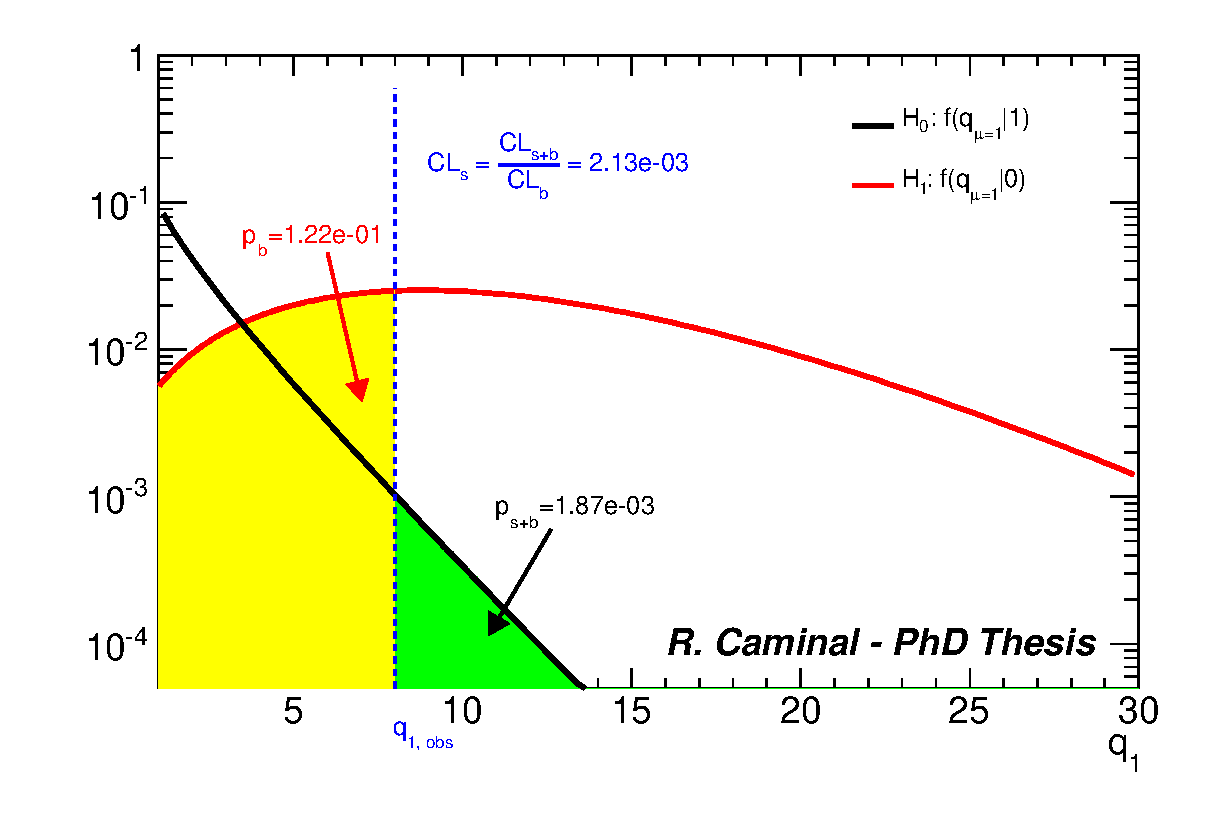
\includegraphics[width=0.75\textwidth]{MonojetAnalysis/Figures/pdfTestHypothesisExample.eps}
    }
  \end{center}
  \caption[Illustration of the PDF of $q_{\mu}$ under the signal plus background and background-only hypotheses.]{Illustration of the PDF of $q_{\mu=1}$ under two different hypothesis: signal plus background (null, $\mu=1$) and background-only (alternative, $\mu=0$). The $CL_{s+b}$, $CL_b$ and $CL_s$ are also shown for this particular example.}
  \label{fig:pdfTestStatisticExample}
\end{figure}

In the work presented in this thesis, the $CL_s$ is calculated for each signal model under evaluation.
The models for which $CL_s < 0.05$, are excluded at 95\% CL.
With the $CL_s$ method, $CL_s \approx CL_{s+b}$ in the cases where the analysis is sensitive to the signal process under study.
Instead, in the cases where the analysis is insensitive, $CL_b$ is be small, thus increasing the value of $CL_s$ and therefore avoiding the exclusion of the signal model.
